\documentclass[a4paper,12pt]{ctexbook}
\usepackage{fontspec}
\setmainfont{Noto Serif CJK SC}
\usepackage{graphicx}
\usepackage{listings,array,tabularx,booktabs,multirow,multicol}
\usepackage{tikz}
\usepackage{tikzsymbols}

% Defining a new coordinate system for the page:
%
% --------------------------
% |(-1,1)    (0,1)    (1,1)|
% |                        |
% |(-1,0)    (0,0)    (1,0)|
% |                        |
% |(-1,-1)   (0,-1)  (1,-1)|
% --------------------------
\makeatletter
\def\parsecomma#1,#2\endparsecomma{\def\page@x{#1}\def\page@y{#2}}
\tikzdeclarecoordinatesystem{page}{
	\parsecomma#1\endparsecomma
	\pgfpointanchor{current page}{north east}
	% Save the upper right corner
	\pgf@xc=\pgf@x%
	\pgf@yc=\pgf@y%
	% save the lower left corner
	\pgfpointanchor{current page}{south west}
	\pgf@xb=\pgf@x%
	\pgf@yb=\pgf@y%
	% Transform to the correct placement
	\pgfmathparse{(\pgf@xc-\pgf@xb)/2.*\page@x+(\pgf@xc+\pgf@xb)/2.}
	\expandafter\pgf@x\expandafter=\pgfmathresult pt
	\pgfmathparse{(\pgf@yc-\pgf@yb)/2.*\page@y+(\pgf@yc+\pgf@yb)/2.}
	\expandafter\pgf@y\expandafter=\pgfmathresult pt
}
\makeatother

\usepackage{lettrine}

\usepackage[absolute]{textpos}
%\usepackage[grid=true,gridcolor=red,subgridcolor=green]{eso-pic}
%\usepackage{eso-pic}
%\usepackage{pict2e,showframe,xcolor}
%\AddToShipoutPictureFG{
%	\AtPageUpperLeft{%
%		\raisebox{-\height}{%
%			\fbox{页心}%
%		}%
%	}%
%	\AtPageCenter{%
%	\raisebox{-\height}{%
%		\fbox{页心}%
%		}%
%	}%
%}

\usepackage{titlesec}
\titleformat{\section}[frame]
{\normalfont}
{\filright
	\footnotesize
	\enspace  \thesection\enspace}
{8pt}
{\Large\bfseries\filcenter}
\titleformat{\chapter}[frame]
{\normalfont}
{\filright
	\footnotesize
	\enspace 第{\Large\color{blue}{\thesection}}回 \enspace}
{8pt}
{\Large\color{green}\bfseries\filcenter}

\usepackage{fancyhdr}
\pagestyle{fancy}
\renewcommand{\chaptermark}[1]{\markboth{#1}{}}
\renewcommand{\sectionmark}[1]{\markright{\thesection\ #1}}
\fancyhf{}
\fancyfoot[C]{\Wintertree\bfseries\thepage\Summertree}
\fancyhead[LO]{\Large\color{red}\bfseries\rightmark}
\fancyhead[RE]{\Large\color{red}\bfseries\leftmark}
\renewcommand{\headrulewidth}{0.4pt} % 注意不用 \setlength
\renewcommand{\footrulewidth}{0pt}

\usepackage{hyperref}
\hypersetup{
  colorlinks   = true, %Colours links instead of ugly boxes
  urlcolor     = blue, %Colour for external hyperlinks
  linkcolor    = blue, %Colour of internal links
  citecolor   = red %Colour of citations
}

\begin{document}

%\author{TeXstudio Team}
%\title{Simple Book Example}
%\date{January 2013}

\frontmatter
%\maketitle
\begin{titlepage}
    \begin{center}
        \vspace*{1cm}
 
        \textbf{Thesis Title}
 
        \vspace{0.5cm}
         Thesis Subtitle
             
        \vspace{1.5cm}
 
        \textbf{Author Name}
 
        \vfill
             
        A thesis presented for the degree of\\
        Doctor of Philosophy
             
        \vspace{0.8cm}
      
        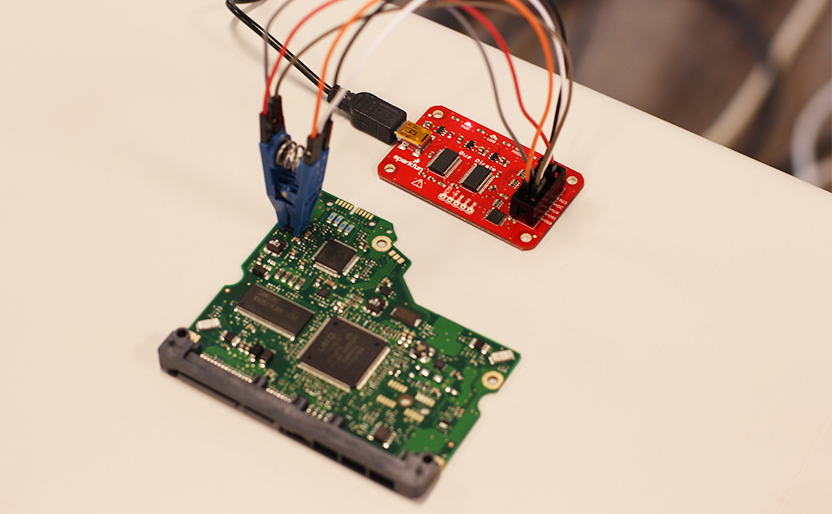
\includegraphics[width=0.4\textwidth]{university}
             
        Department Name\\
        University Name\\
        Country\\
        Date
             
    \end{center}
 \end{titlepage}
\tableofcontents

\mainmatter
\chapter{The First Chapter}

\begin{tabular}{l}
    \hline
    “天地玄黄,宇宙洪荒。日月盈昃,辰宿列张。”\footnotemark \\
    \hline
\end{tabular}
\footnotetext{表格里的名句出自《千字文》。}
    
\marginpar{\footnotesize 边注较窄,不要写过多文字,最好设置较小的字号。}

《木兰诗》:
\begin{quotation}
	万里赴戎机,关山度若飞。
	朔气传金柝,寒光照铁衣。
	将军百战死,壮士十年归。
	
	归来见天子,天子坐明堂。
	策勋十二转,赏赐百千强。......
\end{quotation}

\begin{quote}
	万里赴戎机,关山度若飞。
	朔气传金柝,寒光照铁衣。
	将军百战死,壮士十年归。
	
	归来见天子,天子坐明堂。
	策勋十二转,赏赐百千强。......
\end{quote}

\begin{verse}
	万里赴戎机,关山度若飞。
	朔气传金柝,寒光照铁衣。
	将军百战死,壮士十年归。
	
	归来见天子,天子坐明堂。
	策勋十二转,赏赐百千强。......
\end{verse}

\begin{verbatim}
#include <iostream>
int main()
{
  std::cout << "你好,高那德!"
  << std::endl;
  return 0;
}
\end{verbatim}

\begin{verbatim*}
#include <iostream>
int main()
{
  std::cout << "你好,高那德!"
  << std::endl;
  return 0;
}
\end{verbatim*}

\verb|\LaTeX| \\
\verb+(a || b)+ \verb*+(a || b)+


\begin{lstlisting}
for i:=maxint to 0 do
begin
{ 做点啥 }
end;
Write(’Case insensitive ’);
WritE(’Pascal keywords.’);
\end{lstlisting}


基线
\begin{tabular}{|c|}
	表腰\\
	与基线对齐\\
\end{tabular}
\begin{tabular}[t]{|c|}
	表头\\
	与基线对齐\\
\end{tabular}
\begin{tabular}[b]{|c|}
	表脚\\
	与基线对齐\\
\end{tabular}
基线\par

下一段:万里赴戎机,关山度若飞。
朔气传金柝,寒光照铁衣。
将军百战死,壮士十年归。

\def\夏树{\Summertree}
\夏树

\begin{tabular}{|@{\Springtree}r@{} @{:}l r@{\Wintertree}|}
	\hline
	1 & 1 & 一 \\
	11 & 3 & 十一 \\
	\hline
\end{tabular}

\begin{tabular}
	{>{\centering\arraybackslash}p{9em}}
	\hline
	万里赴戎机,关山度若飞。
	朔气传金柝,寒光照铁衣。 \\
	\hline
\end{tabular}

\newcommand\木兰辞{万里赴戎机}

\begin{tabular}{cp{2em}m{2em}b{2em}}
	\hline
	基线 & \木兰辞 & \木兰辞 & \木兰辞 \\
	\hline
\end{tabular}

\begin{tabularx}{14em}%
	{|*{5}{>{\centering\arraybackslash}X|}}
	\hline
	甲 & 乙 & 丙 & 丁 & 戊 \\ \hline
	己 & 庚 & 辛 & 壬 & 癸 \\ \hline
\end{tabularx}

\begin{tabular}{|c|c|c|}
	\hline
	4 & 9 & 2 \\ 
	\cline{2-3}
	3 & 5 & 7 \\ 
	\cline{1-1}
	8 & 1 & 6 \\ 
	\hline
\end{tabular}

\begin{tabular}{cccc}
	\toprule
	& \multicolumn{3}{c}{数字} \\
	\cmidrule{2-4}
	& 1 & 2 & 3 \\
	\midrule
	Alphabet & A & B & C \\
	Roman
	& I & II& III \\
	\bottomrule
\end{tabular}

\begin{tabular}{cccc}
	\hline\\
	& \multicolumn{3}{c}{数字} \\
	\cmidrule{2-4}
	& 1 & 2 & 3 \\
	\hline\\
	字母 & A & B & C \\
	欧数
	& I & II& III \\
	\hline\\
\end{tabular}

\begin{tabular}{|*{3}{c|}}
	\hline
	甲 & 乙 & 丙 \\\hline
	\multicolumn{2}{|c|}{甲乙} & \multicolumn{1}{r|}{丁}\\\hline
	甲 & \multicolumn{2}{c|}{乙丙} \\\hline
\end{tabular}

\begin{tabular}{ccc}
	\hline
	\multirow{2}{*}{项} & \multicolumn{2}{c}{值}\\
	\cline{2-3}
	& 首 & 末 \\ \hline
	甲 & 乙 & 丙 \\\hline
\end{tabular}

|\mbox{ 庚、辛、壬、癸}|\\
|\makebox[10em]{ 庚、辛、壬、癸。}|\\
|\makebox[10em][l]{ 庚、辛、壬、癸。}|\\
|\makebox[10em][r]{ 庚、辛、壬、癸。}|\\
|\makebox[10em][s]{ 庚、辛、壬、癸。}|

\framebox[10em][r]{测试盒。}\\[1ex]
\setlength{\fboxrule}{1.6pt}
\setlength{\fboxsep}{1em}
\framebox[10em][r]{\phantom{测}}
\framebox[10em][r]{测试盒。}

三字经:\parbox[t]{3em}%
{人之初 性本善 性相近 习相远}
\quad
千字文:\lower0.4ex\hbox{
\begin{minipage}[b][2ex][t]{4em}
	天地玄黄 宇宙洪荒
\end{minipage}}

\meaning\XeteX

微页\fbox{\begin{minipage}{15em}%
		这是一个垂直盒子的测试。
		\footnote{脚注来自 微页。}
\end{minipage}}

黑 \rule{12pt}{4pt} 盒.
上些 \rule[4pt]{6pt}{8pt} 与
下些 \rule[-4pt]{6pt}{8pt} 盒.
一条 \rule[-.4pt]{3em}{.4pt} 线.
\hrule

\TPGrid[0mm,0mm]{10}{10}
\TPShowGrid{10}{10}

\begin{textblock}{1}(0,0)
\textblocklabel{第二块}
任意位置放文本。
\end{textblock}

\begin{tikzpicture}[remember picture,overlay,every node/.style={anchor=center}]
\node at (page cs:0.5,0.3) {0.5,0.3};
\node at (page cs:-0.25,0.3) {-0.25,0.3};
\node at (page cs:0,0) {0,0};
\draw(page cs:-0.25,0) -- (page cs:.75,-0.5);
\draw[thick] (page cs:-1,-1) rectangle (page cs:1,1);
\end{tikzpicture}

\lettrine[lines=3,lhang=0.2,loversize=0.25]{关}{山}度若飞


\chapter{The Second Chapter}

\AddToShipoutPictureBG*{% on the background, only this page
	\AtTextUpperLeft{%
		\put(30mm,-25mm){\color{lightgray}\circle*{50}\quad 前景○}
		
	}
}
\AddToShipoutPictureFG*{% on the foreground, only this page
	\AtTextUpperLeft{%
		\put(60mm,-25mm){\color{blue}\circle*{50}}
	}
}

\AddToShipoutPictureBG*{%
	\AtTextCenter{%
		\makebox(0,0)[c]{\resizebox{\textwidth}{!}{%
		\rotatebox{45}{\textsf{\textbf{\color{lightgray}草稿}}}}}
	}
}

文本内的图片不会换行直接出去了
\setlength{\unitlength}{1.6cm}
\begin{picture}(6,5)
\thicklines
\put(1,0.5){\line(2,1){3}}
\put(4,2){\line(-2,1){2}}
\put(2,3){\line(-2,-5){1}}
\put(0.7,0.3){$A$}
\put(4.05,1.9){$B$}
\put(1.7,2.95){$C$}
\put(3.1,2.5){$a$}
\put(1.3,1.7){$b$}
\put(2.5,1.05){$c$}
\put(0.3,4){$F=\sqrt{s(s-a)(s-b)(s-c)}$}
\put(3.5,0.4){$\displaystyle s:=\frac{a+b+c}{2}$}
\put(0,0){\color{red}\circle*{0.1}(0,0)}
\put(6,0){\color{red}\circle*{0.1}(6,0)}
\put(0,5){\color{red}\circle*{0.1}(0,5)}
\put(6,5){\color{red}\circle*{0.1}(6,5)}
\end{picture}

{\fontsize{50}{50}\selectfont 大}江东去
{\tiny 微}{\scriptsize 细}{\footnotesize 注}{\small 小}{\normalsize 常}{\large 大}{\Large 更大}{\LARGE 特大}{\huge 巨}{\Huge 更巨}

\sffamily
文字用\textcolor{red}{红色}强调\\
\colorbox[gray]{0.95}{浅灰色背景} \colorbox[rgb]{0.5,0.5,0}{\hspace{10em}\phantom{色}}\\
\fcolorbox{blue}{yellow}{%
	\textcolor{blue}{蓝色边框+文字,%
		黄色背景}
}

\begin{tikzpicture}
\node[circle,fill=blue,text=white,
node font={\bfseries}]
(甲) at (-2,0) {节点};
\node[rectangle,rounded corners,
draw=gray,
node font={\sffamily\slshape}]
(①) at (2,0) {框数};
\end{tikzpicture}

\begin{tikzpicture}[remember picture,overlay]
\foreach \bound in {north,south,west,east,45} {
	\node[anchor=\bound] at (current page.\bound) {I am \bound-bound...};
}
\node at (current page.center) {I am NOT MOOVING!};
% You can see the border of the page node with this:
\draw[thick] (current page.south west) rectangle (current page.north east);
\end{tikzpicture}

\backmatter
% bibliography, glossary and index would go here.

\end{document}